%%%%%%%%%%%%%%%%%%%%%%%%%%%%%%%%%%%%%%%%%%%%%%%%%%%%%%%%%%%%%%%%%%% 
%                                                                 %
%                            CHAPTER ONE                          %
%                                                                 %
%%%%%%%%%%%%%%%%%%%%%%%%%%%%%%%%%%%%%%%%%%%%%%%%%%%%%%%%%%%%%%%%%%% 
 
\chapter{Introduction}
 
\section{Motivation}
The thesis is interested in solving engineering design optimization problems that are governed by Partial-Differential-Equations (PDEs). Such PDE-constrained optimization problems arise in many engineering applications including aerodynamic shape optimization \cite{lambe:2014,lyu2014aerodynamic, Zhang567303}, structural optimization \cite{DBLP:DeckelnickHJ17, lambe:2014, kennedy14}, and thermodynamic optimization \cite{chen1999finite,bejan2000thermodynamic,bejan2012thermodynamic}.  %


\begin{figure}[H]
\centering
\subfloat[Aero-Structure Optimization~\cite{as_opt}]{
  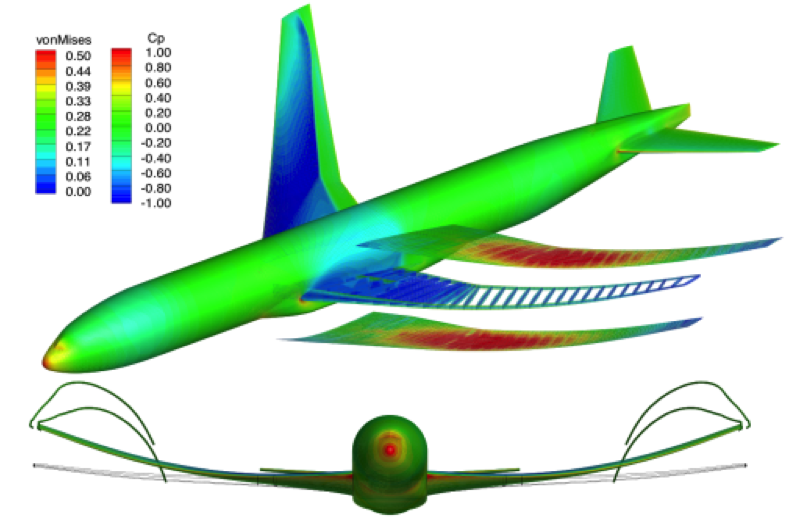
\includegraphics[clip,width=0.5\columnwidth]{./figs/1_as.png}\label{fig:A}  %
}
\subfloat[Topology Optimization~\cite{topo_opt}]{ %
  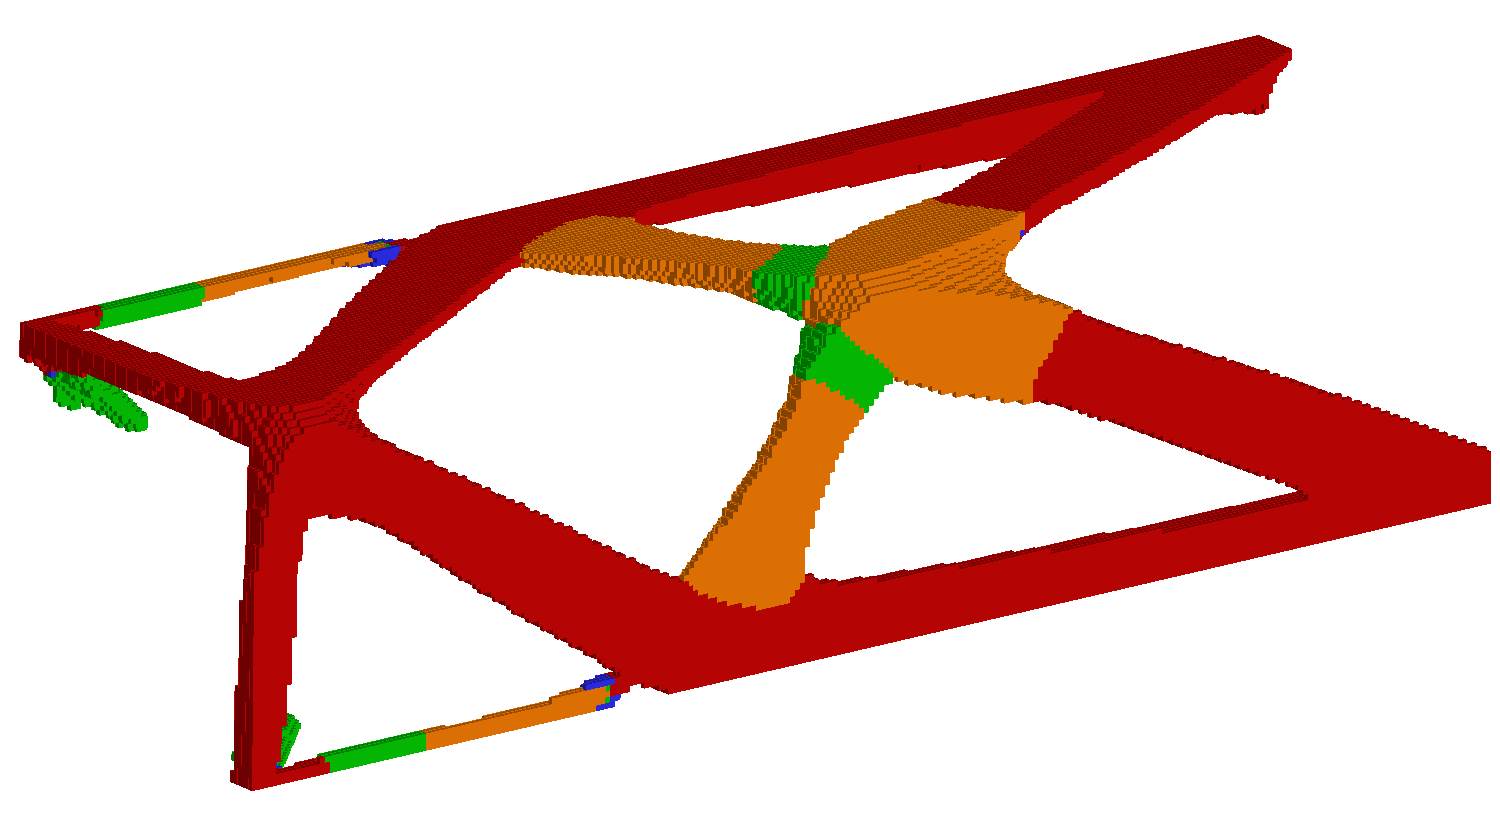
\includegraphics[clip,width=0.5\columnwidth]{./figs/1_topo.png}\label{fig:B}
}
\caption{Large-Scale PDE-constrained Optimization}
\label{fig:1_mot}
\end{figure}

In such applications, an optimization library is coupled with a PDE solver. The simulation problem solves the PDEs for state variables, e.g. the pressure distribution along the surface mesh node points on the wing in Figure~\ref{fig:A}, the displacement distribution among the solid mesh node points in Figure~\ref{fig:B}, at certain design variables. The performance of the physics system is evaluated in the form of objective function given certain constraints, and the objective and some of the constraints are computed via the state variables. The optimizer will choose a design point, request the PDE solver for state variables, and compute the functional values and the gradients at that point. The optimizer will process all the information and yield a better design point using detailed mathematical algorithms. The process is repeated until certain criteria is met for optimality.  

The optimization framework is simple, and has been used successfully in many application fields. The difficulty in PDE-constrained optimization is that the PDE solution (or state equation), which itself is a complicated topic to which intensive effort has been devoted, is just a subproblem of the optimization problem. In large-scale engineering, the PDE solve and gradient evaluation can be very expensive. In addition, storing the necessary matrix or vectors 


can be very demanding.  To find the optimal design, the optimizer may request the PDE solution and calculate the gradients for many different design points, and will need to store a certain amount of large state vectors.    

General-purpose optimization algorithms are unsuitable, because their matrix-based approaches need to compute the total constraint Jacobians as well as store them, resulting in poor scalability performance. In addition, their limited-memory quasi-Newton methods have linear asymptotic convergence rates. For large-scale optimization problems with thousands of design variables or constraints, the computational cost is unmanageable.

This thesis intends to address these challenges by proposing a scalable optimization framework specially for large-scale PDE-constrained design problems. 

\section{Solving PDE-constrained Optimization Problem}
A generic PDE-constrained optimization problem can be stated as
\begin{equation}\label{eq:gen1}
\begin{aligned}
\underset{x,u}{\text{min}} \quad &f(x, u) &\\
\text{subject to} \quad &  h(x,u) &= 0  \\
 &  g(x,u) &\geq 0  \\
\text{governed by} \quad &  \mathcal{F}(x, u) &= 0, \\
\end{aligned}
\end{equation}
where $x \in \mathbb{R}^n, u \in \mathbb{R}^v$ are the design and state vectors respectively, and $f: \mathbb{R}^n \rightarrow \mathbb{R}, h: \mathbb{R}^n \rightarrow \mathbb{R}^l, g:\mathbb{R}^n \rightarrow \mathbb{R}^m$ are the objective, equality and inequality constraints respectively. We assume that $f$, $h$ and $g$ have continuous second derivatives. 

The challenge in solving \eqref{eq:gen1} is that general-purpose gradient-based optimization algorithms \cite{Nocedal2006NO, Byrd:1999:IPA:588897.589167,gill:2002} require the total derivative of the objective and constraints with respect to the design variables, and each of these total derivatives requires the solution of an $v\times v$ linear system, \ie a discretized PDE.  For example, the total derivative of the $i$th constraint $g_i$ is given by
\begin{align}
\frac{d}{dx}\left(g_i\right) &= \frac{\partial}{\partial x}\left(g_i\right) + \psi ^T \left[ \frac{\partial}{\partial x}\mathcal{F} \right] \\
\intertext{where $\psi \in \mathbb{R}^v$ is the adjoint which is governed by the discretized PDE,}
\left[ \frac{\partial}{\partial u}\mathcal{F} \right]^T \psi &= - \frac{\partial}{\partial u}\left(g_i\right) 
\end{align}
which is the adjoint equation \cite{Jameson03aerodynamicshape}. The computational cost of solving the adjoint equation is equivalent to that of the PDEs governing equation. Clearly, if the number of constraints $m$ is sufficiently large, it will be prohibitively expensive to compute all the total derivatives for optimization as each one entails an adjoint. 

To solve \eqref{eq:gen1}, the Lagrangian formulation is:
\begin{equation}\label{eq:lag}
\mathcal{L}(x, u, \psi, s, \lambda_h, \lambda_g) = f(x,u) + \lambda_h^T h(x, u) + \lambda_g^T (g(x,u)-s) + \psi^T \mathcal{F}(x,u),
\end{equation} 
where $s \in \mathbb{R}^m$ is for transforming the inequality constraints into equality ones, and $\lambda_h \in  \mathbb{R}^l$,  $\lambda_g \in  \mathbb{R}^m$ are the Lagrangian multiplier vectors for equality and inequality constraints. 

The first-order optimality conditions, or the \textit{Karush-Kuhn-Tucker} (KKT) conditions for \eqref{eq:gen1} are derived by taking partial derivatives of 
\eqref{eq:lag} with respect to all the unknown variables,
\begin{equation}\label{eq:kktcond}
\begin{aligned}
\nabla_x \mathcal{L} &= \nabla_x f + \lambda_h^T \nabla_x h + \lambda_g^T \nabla_x g + \psi^T \nabla_x\mathcal{F} = 0, \\
\nabla_u \mathcal{L} &= \nabla_u f + \lambda_h^T \nabla_u h + \lambda_g^T \nabla_u g + \psi^T \nabla_u\mathcal{F} = 0, \\
\nabla_{\psi} \mathcal{L} &= \mathcal{F} = 0, \\
\nabla_{\lambda_h} \mathcal{L} &= h = 0, \\
\nabla_{\lambda_g} \mathcal{L} &= g - s = 0, \\
-\mathcal{S} \Lambda_g e &= 0,\\
s \geq 0, &\quad \lambda_g \leq 0. \\
\end{aligned}
\end{equation}

The big nonlinear systems of equations \eqref{eq:kktcond} can be solved in either the full space or the reduced space.  Full-space methods~\cite{DBLP:journals/siamsc/BirosG05,DBLP:journals/siamsc/BirosG05a,haber:2001} solve all the unknowns in \eqref{eq:kktcond} simultaneously. The resulted KKT system is large, more than two times the number of state variables, indefinite and ill-conditioned. During optimization iterations, the state equation $\mathcal{F} =0$ and adjoint equation $\nabla_u \mathcal{L} = 0$ do not need to be solved exactly, avoiding the computational expense of tightly converging the PDE and adjoint equation residuals; however, this is also a potential disadvantage in practical engineering problems, because, if the optimization fails to converge, the intermediate solution may not be feasible with respect to the physics.  Furthermore, for highly nonlinear PDEs, \eg gas dynamics with shocks and boundary layers, practitioners have developed specialized globalization strategies that may be difficult to take advantage of in general-purpose full-space optimization algorithms.

In contrast, reduced-space algorithms treat the states $u$ and the adjoints $\psi$ as implicit functions of the design variables through $\mathcal{F}(x,u(x)) = 0$, $\nabla_u \mathcal{L} = 0$. The reduced KKT condition is formulated as follows, 
\begin{equation}\label{eq:opt00x}
 \begin{gathered}
    F(x,s,\lambda_h, \lambda_g) \equiv 
    \begin{bmatrix}
\nabla_x f + \lambda_h^T \nabla_x h + \lambda_g^T \nabla_x g\\
-\mathcal{S} \Lambda_g e\\
h  \\
g - s 
\end{bmatrix} =0,\\
\text{subject to} \quad s_i \geq 0, \quad \text{and} \lambda_{gi} \leq 0. \\
\end{gathered}
\end{equation}

where $s \in \mathbb{R}^m$ denotes the slack variables, $q \equiv (x^T, s^T,
\lambda_h^T, \lambda_g^T) \in \mathbb{R}^{N}$ is a vector of all the unknowns,
and $F :\mathbb{R}^{N} \rightarrow \mathbb{R}^{N}$ is the vector-valued residual
of the KKT conditions excluding the inequalities on $s$ and $\lambda_g$.  For
convenience, we have also introduced $e = [1,1,\ldots,1]^T$ and the diagonal
matrices
\begin{equation*}
  \mat{S} = \mydiag\left(s_1,s_2,\ldots,s_m\right),\qquad\text{and}\qquad
  \mat{\Lambda_g} = \mydiag\left(\lambda_{g1}, \lambda_{g2}, \ldots, \lambda_{gm}\right).
\end{equation*}


Therefore, the resulted KKT system is much smaller, and it can make use of existing PDE solvers and adjoint solvers, maintaining modularity. Reduced-space methods have been successfully implemented in unconstrained problems and IDF problems. The unconstrained version of \eqref{eq:opt00x} can be solved efficiently using a Newton-Krylov (NK) algorithm applied to the first-order optimality conditions; see, for example, \cite{akcelik:2006, Heinkenschloss:1999:IOA, hinze2010optimization,borzi:2011}. NK optimization algorithms have also shown promise for equality-constrained optimization in the reduced space, because they do not require the constraint Jacobian to be form explicitly and, thus, avoid the scaling issue described earlier.  For instance, \cite{dener:idf2017} applied a matrix-free NK algorithm to a class of equality-constrained optimization problems that arise in multidisciplinary design optimization and would otherwise be intractable with conventional matrix-based algorithms.

Motivated by its success in the unconstrained and equality-constrained cases, we would like to extend the Newton Krylov methodology to more general, inequality constrained problems, to solve \eqref{eq:opt00x}. 

\section{Inexact-Newton Methods}

An alternative to using conventional (matrix-based) optimization algorithms or
constraint aggregation is to apply inexact-Newton methods~\cite{dembo:1982},
also know as truncated-Newton methods in the optimization
literature~\cite{nash:2000} to solve \eqref{eq:opt00x}.  

With the exception of the bounds on $s$ and $\lambda_g$, the KKT conditions
\eqref{eq:opt00x} form a set of nonlinear algebraic equations, $F(q)=0$.  These
equations can be solved, in principle, using Newton iterations of the form
\begin{equation}
(\nabla_q F) \Delta q^{(k)} = -F(q^{(k)}), \label{eq:Newton}
\end{equation}
where $q^{(k)}$ is the solution at the $k$th iteration and $\Delta q^{(k)} =
q^{(k+1)} - q ^{(k)}$ is the solution update.  Solving~\eqref{eq:Newton} exactly
can be inefficient during early Newton iterates when the linear model is not a
good approximation to $F(q)=0$.  Instead, truncated- and inexact-Newton methods
find approximate solutions to \eqref{eq:Newton} that, for example, satisfy the
inexact-Newton condition
\begin{equation}
  \left\| (\nabla_q F) \Delta q^{(k)} + F(q^{(k)}) \right\| \leq \eta_k \left\| F(q^{(k)}) \right\|, \label{eq:inexact_Newton}
\end{equation}
for some parameter $\eta_k \in (0,1)$.

There has been considerable success applying inexact-Newton methods to
unconstrained optimization problems; see \cite{nash:2000} and the references
therein.  On the other hand, inexact-Newton methods for general (nonconvex)
constrained problems are much less common.  Some notable exceptions include the
efforts by Byrd and colleagues~\cite{byrd:2008, byrd:2010} and by Heinkenschloss
and Ridzal~\cite{heinkenschloss:2014}; however, these algorithms make
assumptions regarding the structure of the problem that favor full-space
formulations, and our experience applying them to reduced-space PDE-constrainted
optimization has been disappointing.

Applying Newton's method to \eqref{eq:opt00x}, the KKT system, also called primal-dual system is obtained:
\begin{equation}\label{eq:kkt0}
\begin{bmatrix} \nabla_{xx} \mathcal{L} & 0 & \mathcal{A}_{h}^T & \mathcal{A}_{g}^T \\
    0 & -\mathcal{S} \Lambda_g & 0 & -\mathcal{S} \\
    \mathcal{A}_{h} & 0 & 0 & 0 \\
    \mathcal{A}_{g} & -\mathcal{S} & 0 & 0 
    \end{bmatrix}
    \begin{bmatrix} p_x \\ \tilde{p_s} \\ p_h \\ p_g \end{bmatrix}
    = - \begin{bmatrix} \nabla_x \mathcal{L} \\ -\mathcal{S} \Lambda_g e \\ h \\ g - s \end{bmatrix}
\end{equation}
where $\mathcal{L}$ the Lagrangian is defined in \eqref{eq:lag}, $\mathcal{S}$ and $\Lambda_g$ are as defined previously. 

NK method solves \eqref{eq:kkt0} using Krylov method, and thus only need the matrix-vector product of the system matrix. However, while NK methods can avoid the cost associated with forming the explicit constraint Jacobian, this extension faces several significant challenges. First, active-set and interior-point algorithms that make use of an explicit basis for the null space of the constraint Jacobian cannot be used, because such a basis requires the Jacobian to be explicitly available.  Second, the primal-dual saddle-point system raised in optimization is indefinite and ill-conditioned, making it difficult for iterative Krylov methods to converge to a sufficient tolerance, hurting the convergence rate of Newton's method. Third, dealing with nonconvex Hessian of the Lagrangian in the null space of the constraint Jacobian is also a non-trivial task. 

The formula \eqref{eq:kkt0} takes the same form as the classical interior point method in Chapter 19 in Nocedal's book \cite{Nocedal2006NO}, which will be reviewed below. 

\section{Review on Interior Point Method  }
The difficulty in extending the Newton Krylov methods to handle inequality constraints, to solve \eqref{eq:opt00x} lies in the nonlinear complementarity condition: for each inequality constraint, either the slack or Lagrangian multiplier is strictly zero if we assume strict complementarity is satisfied at the solution. The slack has to be non-negative to guarantee feasibility of the inequality constraints, and the multipliers has to be non-positive in respect to the property of a local minimization point following the formula convention. For inequality constraints that are active at the solution, slack variable is zero and the multiplier is negative, while for inactive inequality constraints, slack variable is positive and the multiplier is negative. Therefore, the complementarity condition, in combined with the sign requirement on slack and multipliers, contains information on optimal active set of the inequality constraints at the solution.   

Currently there are two most powerful algorithms for general nonlinear constrained problems: active-set SQP methods and interior point methods \cite{Nocedal2006NO}. Determining the inequality constraint sets that are active at the solution is the main challenge facing active-set methods. Especially when the number of inequality constraints is large, the method may need many iterations to locate the active-set of inequality constraints. While for interior point methods, there are two varieties based on globalization strategies: Newton-Lagrangian line-search and trust-region SQP on the barrier problems. The former is more for illustration purpose, and the latter is actually implemented in practical optimization software libraries IPOPT \cite{W�chter2006}, and KNITRO \cite{Byrd:1999:IPA:588897.589167}. 

The trust-region SQP method builds a quadratic model on the barrier formulation, employs direct linear algebra, uses explicit constraint Jacobians to first compute the multipliers that deliver minimum linearized constraint violations, then compute the design and slack update steps that minimize the quadratic model. In both subproblems, a trust region bound is imposed on the design and slack components, with the slack variable scaled properly to prevent it away from the nonnegative bound. A proper merit function mimic the quadratic objective function is used to estimate the quality of the steps and control the trust-region radius for next iteration. 

To handle nonlinearities and nonconvexities, regularization terms can be added to the Hessian block and the equality constraint Jacobian on the diagonal of the KKT matrix. The proper amount of regularization is computed at each iteration by trial and error such that the inertia of the regularized KKT matrix is $(n+m, l+m, 0)$, under which condition the total Hessian block of design and slack will be positive definite on the null space of the combined constraint matrix, therefore the resulted Newton step will be a guaranteed descent direction for a large class of merit functions. 

Using the proper barrier parameter $\mu$ updating strategy is crucial to the performance of interior point methods: A slowly decreasing $\mu$ will result in large number of outer iterations, making the algorithm less efficient. While a quickly decreasing $\mu$ may make some slack or inequality multipliers approach zero prematurely, hurting the convergence. Some simple implementations of interior point methods use a constant fraction updating scheme, while some chooses the fraction value based on the recent iterations' progress towards the solution. Making the fraction value close to zero near the solution can yield a superlinear convergence rate. More robust strategies update $\mu$ based on the progress of the current complementarity products. Predictor strategy first calculates a predictor direction by setting $\mu=0$, then calculates the tentative complementarity product along this direction using the step size from fraction to boundary rule. The updating fraction value is based on the ratio of this tentative and current complementarity product. 


The former Newton-Lagrangian line-search method solves a perturbed KKT system at each homotopy parameter, also called the barrier parameter $\mu$:

\begin{equation}\label{eq:kkt1}
\begin{aligned}
\nabla f(x) + \lambda_h^T \nabla h(x) + \lambda_g^T \nabla g(x) &= 0 \\
-\mathcal{S} \Lambda_g - \mu e &= 0\\
h(x) &= 0 \\
g(x) - s &= 0 \\
s \geq 0, \quad &\lambda_g \leq 0 \\
\end{aligned}
\end{equation}
The barrier parameter $\mu$, is a sequence of strictly positive numbers and converges to zero. The perturbed KKT system \ref{eq:kkt1} is solved for each $\mu$, and the solution trajectory converges to the KKT point of the original problem in the limit.  

Newton's method is used to solve \ref{eq:kkt1} for each $\mu$, where each Newton step is as follows:
\begin{equation}
\begin{bmatrix} \mathcal{W} & 0 & \mathcal{A}_{h}^T & \mathcal{A}_{g}^T \\
    0 & -\Lambda_g & 0 & -\mathcal{S} \\
    \mathcal{A}_{h} & 0 & 0 & 0 \\
    \mathcal{A}_{g} & -\mathcal{I} & 0 & 0 
    \end{bmatrix}
    \begin{bmatrix} p_x \\ p_s \\ p_h \\ p_g \end{bmatrix}
    = -\begin{bmatrix} \nabla_x \mathcal{L} \\ -\mathcal{S} \Lambda_g - \mu e  \\ h(x) \\ g(x) - s \end{bmatrix}
\end{equation}
After the Newton step direction is computed, fraction to the boundary rule is applied to determine the maximum allowable step size to keep the slack and inequality multipliers away from the 0 bound. Then a backtracking line search is performed to find the step length that delivers sufficient decrease in the merit function or accepted by the filter. The barrier parameter is then updated for the next iteration. 

There are potential drawbacks when using interior point methods for PDE-constrained optimization. For instance, to ensure progress towards global minimum, either trust-region or line-search globalization techniques have to be implemented. The former judges the quality of a computed step by calculating the merit function value and adjust the trust-region radius accordingly, while the latter computes the step-length along a step direction that satisfies the Wolfe condition. In either case, extra computation is needed. Dealing with nonconvex Hessian of the Lagrangian in the null space of the constraint Jacobian is also a non-trivial task; possible solutions include adding a proper regularization term to enforce a positive definite Hessian, see \cite{hicken:flecs2014} and Algorithm B.1 \cite{Nocedal2006NO}. Moreover, the saddle-point matrix raised in optimization is indefinite and ill-conditioned, making it difficult for iterative Krylov methods to converge. 

% \section{Homotopy Methods}

% \section{Krylov Iterative Method}

% \section{KKT Matrix Vector Products}

\section{Preconditioner}

\section{Tools}

\section{Challenges and Contributions}

Our long-term goal is to develop an efficient inexact-Newton algorithm that is
suitable for reduced-space PDE-constrained optimization problems of the
form~\eqref{eq:gen_reduced}.  This goal faces two significant challenges, which
we seek to address in this work.
\begin{description}
\item[Nonconvexity:] The system $F(q) =0$ does not distinguish between different
  types of stationary points, so a basic Newton's method may converge to local
  maximizers or saddle points.  Conventional optimization algorithms often
  project onto the null-space of the (active) constraint Jacobian to detect
  directions of negative curvature and avoid undesirable stationary points, but
  the null-space is not explicitly available for matrix-free inexact-Newton
  methods.
\item[Preconditioning:] The number of iterations necessary to satisfy the
  inexact Newton condition \eqref{eq:inexact_Newton} using, for example, a
  Krylov method is closely related to the condition number of the system.
  Unfortunately, it is well known that the primal-dual, or KKT, matrix $\nabla_q
  F$ is indefinite and highly ill-conditioned.  A preconditioner is needed that
  is inexpensive to form, factor, and store.  A general-purpose, inexpensive
  preconditioner is especially difficult to find in the reduced-space context,
  since approximations to $\nabla_q F$ are not readily available as they are in
  the full-space.
\end{description}

Our approach to addressing globalization is to introduce a homotopy map that
implicitly defines a solution curve that connects the solution to an easy
problem to the solution of the desired problem.  We then use a
predictor-corrector algorithm to follow the curve from the easy to the desired
solution.  A related globalization is used in \cite{Perez2009homotopy} in the
context of a trust-region managed sequential approximate optimization.  To
address the conditioning of the KKT matrix, we propose a low-rank approximation
of the Schur complement that is constructed by applying a few iterations of the
Lanczos method with approximate adjoints.

%The remaining paper is organized as follows. In Section \ref{sec:homotopy}, we
%review homotopy-based globalization and the homotopy map we adopt in this work.
%Section~\ref{sec:pc} describe our predictor-corrector path-following algorithm
%for tracing the homotopy zero curve.  Section~\ref{sec:matfree} begins by
%reviewing Krylov iterative methods, but the focus of the section is the proposed
%low-rank SVD preconditioner.  Section~\ref{sec:results} includes three test
%problems that verify and demonstrate the algorithm.  Finally,
%Section~\ref{sec:conclude} provides our summary and conclusions.

\newpage

\section{Thesis Objectives and Outline}
The objective of this thesis is to develop a scalable matrix-free optimization algorithm suitable for PDE-constrained design problems, together with proper preconditioners accelerating the convergence of the iterative kernel solver. The objectives are summarized as follows:

\begin{itemize}
  \item Develop an efficient scalable matrix-free optimization algorithm for PDE-constrained optimization problems
  \item Develop proper preconditioners for the iterative solver
  \item Verify the accuracy and scalability of the optimization algorithm on analytical problems
  \item Verify the algorithm and preconditioner on a structural PDE-constrained problems
  \item Verify the algorithm and preconditioner on an aerodynamic shape optimization problem
\end{itemize}

The thesis is organized as follows: Chapter 2 describes the matrix-free optimization algorithm. Chapter 3 describes the preconditioners for the linear system of the algorithm. Chapter 4 verifies the optimization method and preconditioner on constructed problems. Chapter 5 applies the optimization method and preconditioner on a stress-constrained mass-minimization problem. Chapter 6 applies the method and preconditioner on an aerodynamic shape optimization problem. In all the applications, Chapters 4,5,6, the results from the new method are benchmarked with a popular large-scale matrix-based active -set augmented-Lagrangian optimization method SNOPT.  






 
% \begin{table}
% \caption[This is the Caption for Table 1]
%            {This is the Caption for Table 1\cite{thisbook}}
%  Note entry in [] for list of tables; you don't want the citation in the LOT.
% \begin{center}
% \begin{tabular}{lll}
% Here's       & an          & example  \\
% of           & a           & table    \\
% floated      & with        & the      \\
% \verb+table+ & environment & command.
%\end{tabular}
% \end{center}
% \end{table}
 
 
% \subsection{This is a Subsection Heading} 
 
% This is a sentence to take up space and look like text.
% This is a sentence to take up space \cite{anotherbook}.
% This is a sentence to take up space and look like text.
 
% \subsubsection{This is a Subsubsection Heading}
% This is a sentence to take up space and look like text.
% This is a sentence to take up space and look like text.
% Text before the footnote.\footnote{Here's the text of the footnote.}
% Text after the footnote. 
% This is a sentence to take up space and look like text.

%%% Local Variables: 
%%% mode: latex
%%% TeX-master: t
%%% End: 
